\chapter{Screen Layout}
\setcounter{figure}{0}
\setcounter{table}{0}

\label{sec:ScreenLayout}
When OptimumTire is opened the project screen will initially appear as shown in Figure~\ref{fig:ProjectScreen}. From this screen the user can either choose to open an existing project or create a new project. Once one of these is selected the primary OptimumTire screen layout will be displayed.

\begin{figure}[H]
	\centering
		\includegraphics[width=1.0\textwidth]{ProjectScreen.png}
	\caption{Project Screen}
	\label{fig:ProjectScreen}
\end{figure}


The OptimumTire screen layout is shown in Figure~\ref{fig:ScreenLayout}. The screen is divided into three basic sections:

\begin{itemize}
\item	The tire project tree
\item	The data entry form
\item	The worksheets and the associated worksheet tabs
\end{itemize}
{}
\begin{figure}[H]
	\centering
		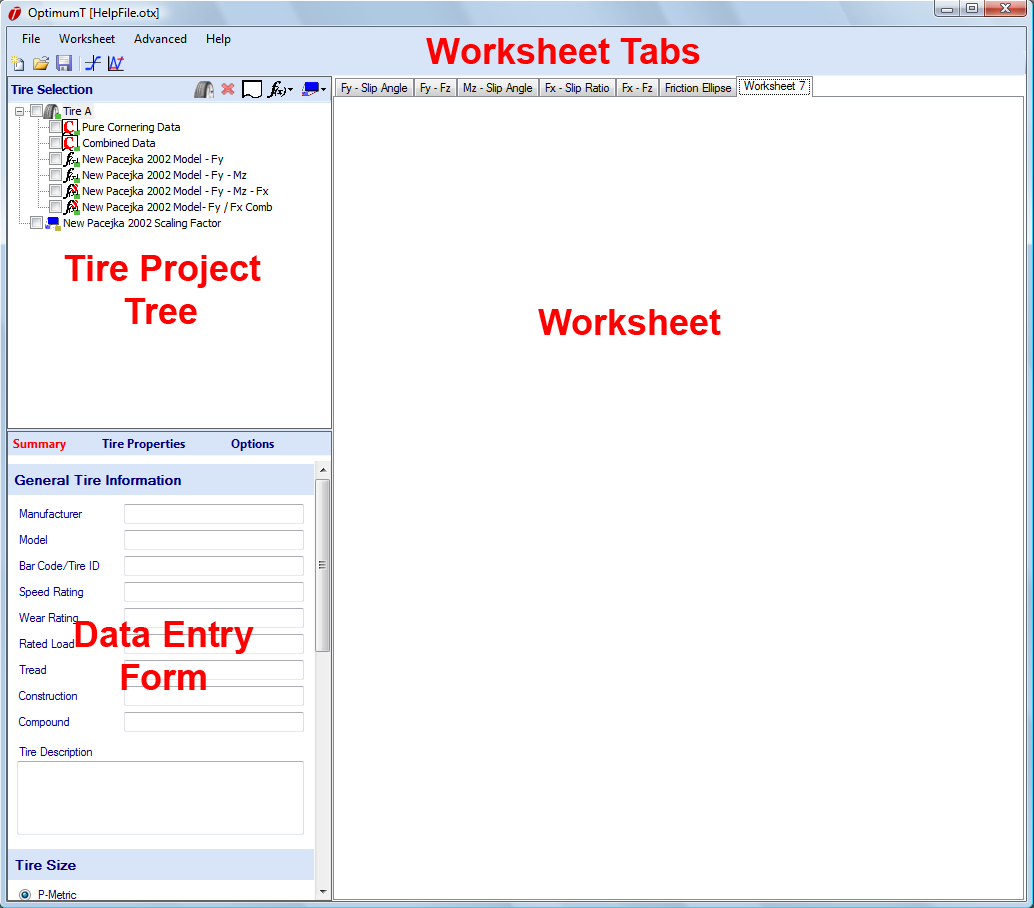
\includegraphics[width=0.95\textwidth]{ScreenLayoutLabeled.png}
	\caption{Screen Layout}
	\label{fig:ScreenLayout}
\end{figure}


\section{Tire Project Tree}
\label{sec:TireProjectTree}
The tire project tree contains all the raw data, tire models, and scaling factors contained within the OptimumTire project. Raw data and tire models are organized by the tire item. The tire items can be seen more closely in Figure~\ref{fig:ProjectTree}.

\begin{figure}[H]
	\centering
		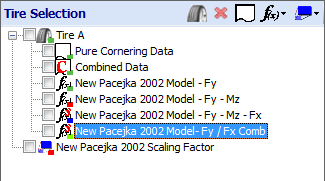
\includegraphics[width=0.95\textwidth]{ProjectTree.png}
	\caption{Project Tree}
	\label{fig:ProjectTree}
\end{figure}

The item type in the project tree can be identified by the icon to the left of the item. In Figure~\ref{fig:ProjectTree}, the first item in the list is a tire. The tire item is like a folder that contains other items in the project. Both raw data and tire models must be associated with a tire item, so this must be the first item added to a new project. This allows data and models from the same tire or construction to be grouped together.

\subsection*{Raw Data}

In Figure~\ref{fig:ProjectTree}, the first two items in the project tree under Tire A are raw data. The icon for the second item, Combined Data, has a large red "C" in it to indicate that the collapsed data is being used. Data collapsing will be explained in section~\ref{sec:DataCollapsing}. 

\subsection*{Tire Models}

The third and fourth items in this project tree are tire models. The next two items are also tire models but the red "S" in the upper right corner of the icon indicates that a scaling factor has been applied to them. 

\subsection*{Scaling Factors}

The final item is a Pacejka scaling factor. These allow the model to be adjusted without making any changes to the model coefficients. Scaling factors are discussed in more detail in section~\ref{sec:ModelScalingFactors}.
 
Like the tire item when any of the raw data, tire models, or scaling factors is clicked additional information and functionality related to the selected item will appear in the data entry form. The small color squares in the lower right corner of the icons indicate the color in which the data or model will be displayed when it is graphed. To graph a specific tire model or raw data set, check the box next to the item in the project tree (graphing is covered in section~\ref{sec:Graphing}).By right clicking on an item you can rename, delete, or copy it as well as perform other operations on it that will be discussed in later sections. 

To add items to the project, the buttons above the project tree can be used. Figure~\ref{fig:ProjectTreeButtons} shows these buttons. The three buttons furthest to the right will only be enabled when an item in the project tree is selected.

\begin{figure}[H]
	\centering
		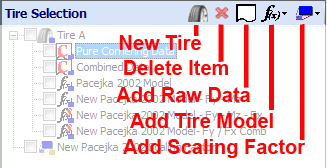
\includegraphics{ProjectTreeButtons.png}
	\caption{Project Tree Buttons}
	\label{fig:ProjectTreeButtons}
\end{figure}

\section{Data Entry Form}
\label{sec:DataEntryForm}
When an item in the project tree is clicked on, a data entry form corresponding to the project item will appear in the data entry area. Note that the name of the project item or its icon must be clicked on. Clicking on the checkbox next to the item in the project tree will not bring up the data entry form, but will change whether or not the item is to be graphed. 

Figure~\ref{fig:TireDataForm} shows an example of the data entry form. This information appears when a tire item is selected in the project tree. Information about the tire size, manufacturing, and testing procedure can be stored here.

If the raw data, tire model, or scaling factor items are selected the information in the data entry area will change to reflect these items. The tire model coefficients are also contained in this form. If a graph is clicked on, the graph setup form for that specific graph will appear in the data entry area. The data entry forms will be discussed in more detail in the chapters corresponding to these specific items.

\begin{figure}[H]
	\centering
		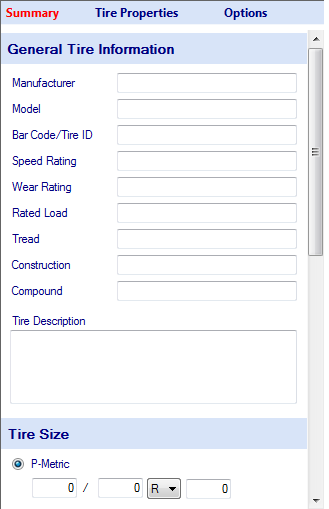
\includegraphics[width=.55\textwidth]{TireDataForm.png}
	\caption{Tire Item Data Entry Form}
	\label{fig:TireDataForm}
\end{figure}

\section{Worksheets}
\label{sec:Worksheets}
The worksheet is the area where graphs can be added to the project. Creating graphs will be covered in section~\ref{sec:Graphing}. An unlimited number of worksheets can be included in a project. To add a new worksheet, click on the \textsl{Worksheet} menu and select \textsl{New Worksheet}. Alternatively, worksheets can be added by right-clicking on the worksheet or the worksheet tabs and selecting \textsl{New Worksheet}.

Worksheets can be renamed by right-clicking on the worksheet and choosing \textsl{Rename Worksheet}. A worksheet can be deleted (and all the graphs on that worksheet) by choosing \textsl{Delete Worksheet} from the menu that appears when you right-click on a worksheet. Note that you cannot undo a delete operation.
